\begin{frame}[allowframebreaks]{Mind > Cognition > Meta cognition}
    \cite{metcalfe-1994-metacognition-knowing-about-knowing} defines metacognition as awareness of one's thought processes and an understanding of the patterns behind them.
    \begin{figure}[H]
        \centering
        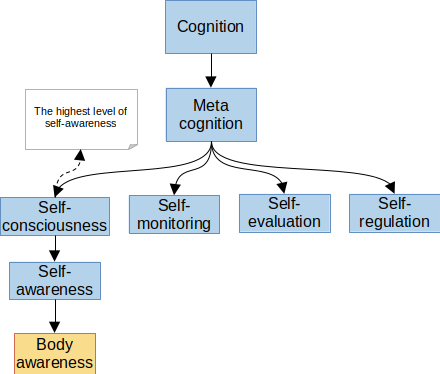
\includegraphics[width=0.5\textwidth]{meta_cognition}
    \end{figure}

    Metacognition is cognition about one's own cognition.
    \begin{itemize}
        \item Having the ability to continuously monitor perceptions and improve them
    \end{itemize}
\end{frame}
